\newpage
\section{Neural Network Architectures}\label{ch:neural_networks}
There are a many different types of neural network architectures. We will talk
about fully-connected, deep, and convolutional neural networks. Some of these
architectures are simpler to implement in practice than others and lend
themselves better to certain types of problems. Remember that image
classification is not the only problem that neural networks are able to solve.

\subsection{Fully-Connected Neural Network} A fully-connected neural network is
a network where all units in one layer are connected to all units in the
following layer. A nonlinear neural network has at least three layers: an input
layer, a hidden layer, and an output layer. Units in the input layer correspond
to the inputs fed into the network. In the case of image classification, this
corresponds to the pixels within each training example.  The output layer's
units correspond to the number of classes an image could fall under. In the
case of both MNIST and CIFAR-10, this number is 10.  A visualization of the
structure of a neural network is shown in Figure \ref{fig:nn} below.

\begin{figure}[ht!]
\centering
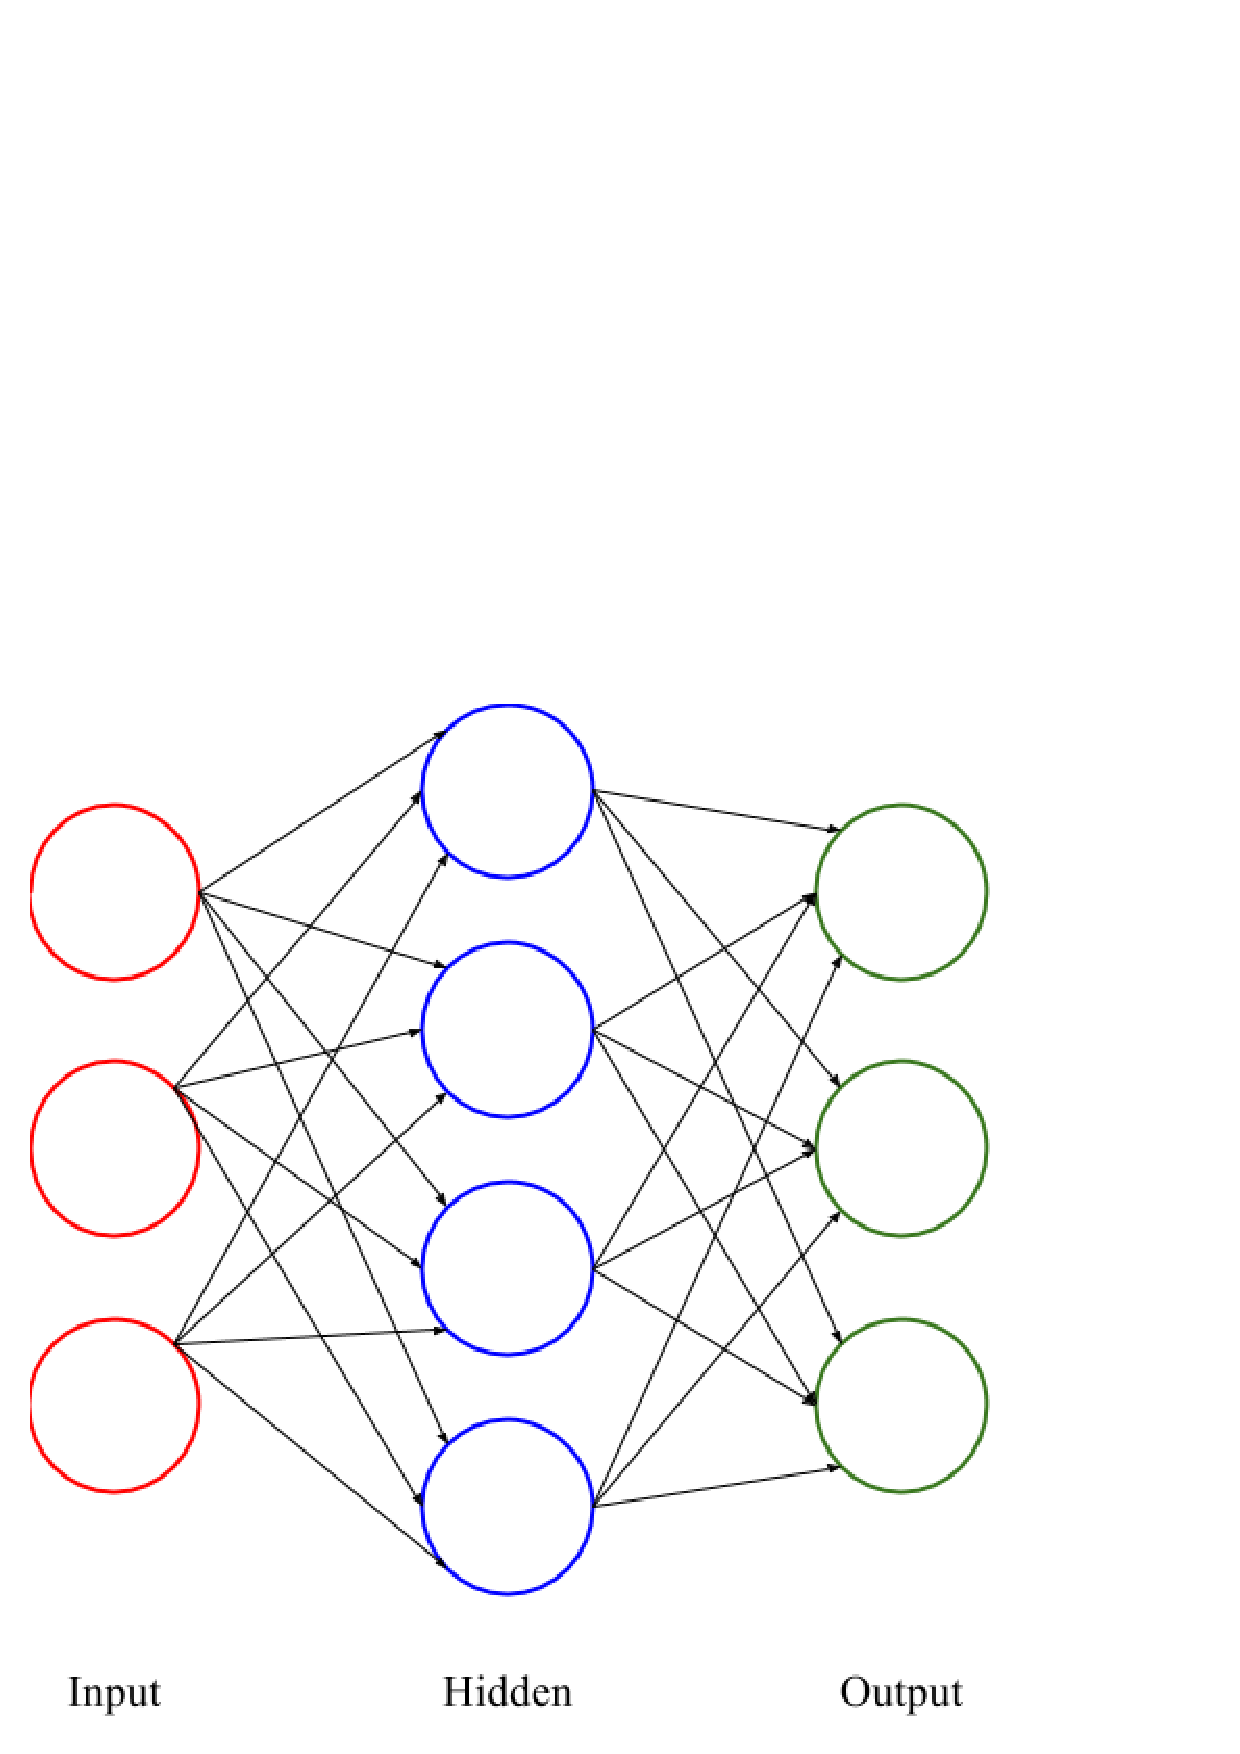
\includegraphics[height=3in]{../figures/neural_network.png}
\caption{Visualization of a fully-connected network.}
\label{fig:nn}
\end{figure}

\subsection{Deep Neural Network}
A neural network can have multiple hidden layers. If it does, it is then
referred to as a deep neural network (DNN). An visualization of a DNN is shown
below.

\begin{figure}[ht!]
\centering
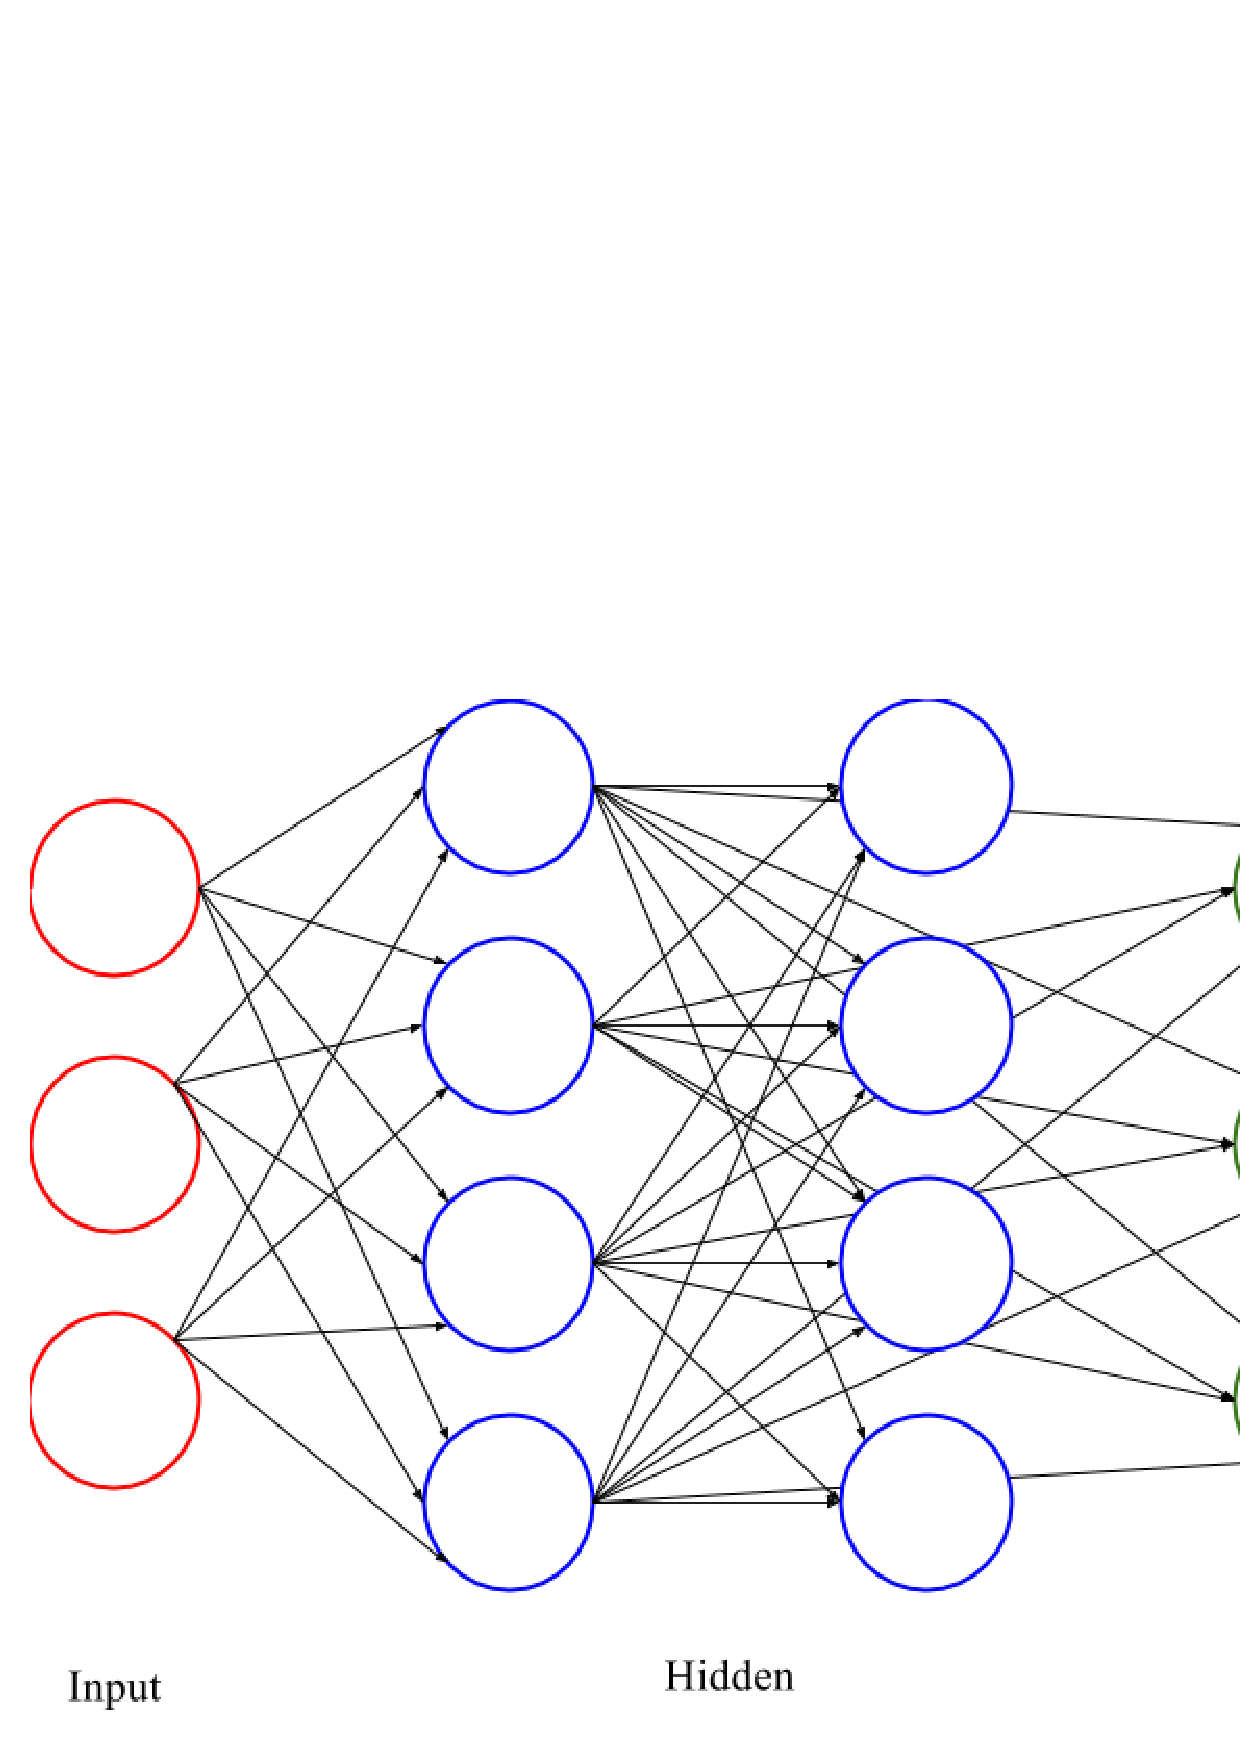
\includegraphics[height=3in]{../figures/deep_nn.png}
\caption{Visualization of a DNN}
\label{fig:dnn}
\end{figure}

We will go into the theory explaining what information each layer of the
network is propogating and explain why multiple layers can achieve better
performance in Chapter \ref{ch:gradient_descent}, but for now, we note that
with multiple hidden layers, information about the images will be learned more
accurately for each iteration of the Gradient Descent algorithm, which is the
algorithm on which a neural network trains. We will discuss this algorithm in
detail later.

\subsection{Convolutional Neural Network}
A convolutional neural network (CNN) is a network where not all units in one
layer are connected to all units in the next. Not all pixels in an image give
useful information about every part of the object they are trying to classify,
so CNNs are commonly used for image classification. They try to avoid
unnecessary computation by removing interactions between units that aren't
providing useful information to each other. A visualization of the structure
of a convolutional neural network is shown in Figure \ref{fig:cnn} below.
\newpage
\begin{figure}[ht!]
\centering
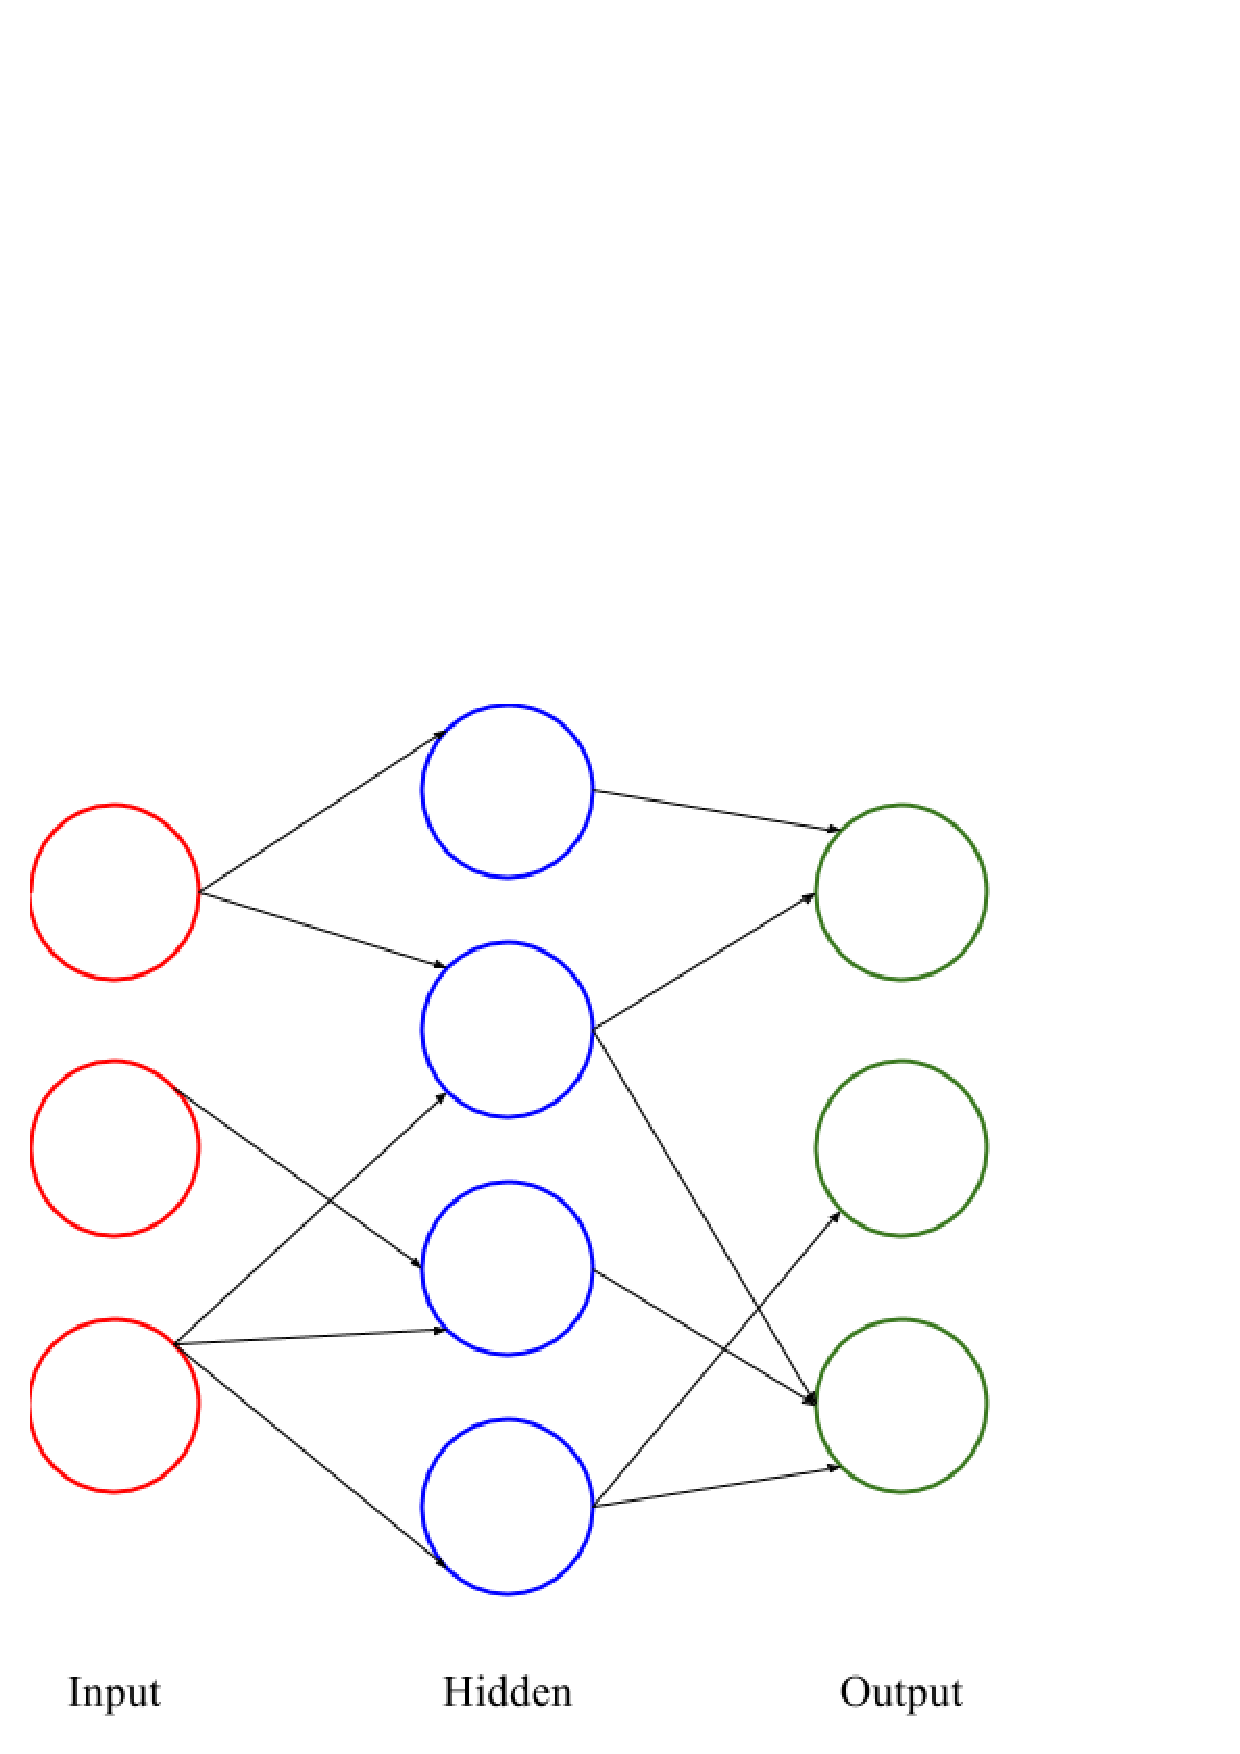
\includegraphics[height=3in]{../figures/convolutional_nn.png}
\caption{Visualization of a CNN}
\label{fig:cnn}
\end{figure}

Note that a CNN can also be a DNN if there are multiple hidden layers. For
image classification, convolutional neural networks tend to perform the best.

\noindent Due to time constraints, this paper will focus exclusively on fully connected
neural networks.
